\chapter{Theoretical Motivation}
\label{chap:theory}
The Standard Model of particle physics describes a set of fundamental particles and their interactions between each other. This description of the SM is a summary of a more detailed understanding found in~\cite{thomson:mpp}. The constituents of the SM can be broadly split into two groups: the fermions, spin-$1/2$ particles which make up all the known matter in the universe, and the bosons, integer spin particles which mediate interactions between the fermions. The fermions are split into the quarks, which are the constituent particles of the proton and neutron, and the leptons, which include the electron. The bosons are responsible for each of the fundamental forces as well as explaining the mass of some particles in the SM.

There are six quarks in total, split into three generations. The first generation consists of the up and the down quark, the second generation is the charm and the strange quark, and the third generation contains the top and the bottom quark. As the generation increases, so do the masses of the quarks. Each generation has a quark with charge +2/3, referred to as up-type quarks, and a quark with charge -1/3, referred to as down-type quarks. Quarks have an additional quantum number referred to as color, which can be red, green, or blue. Each quark also has an antiparticle, which has an anticolor: antired, antigreen, or antiblue. Quarks are hypothesized to obey color confinement: a mechanism that prevents quarks from existing outside of bound, color neutral states. Color confinement seems likely because the nature of gluons indicates that the long-distance strong force between two free quarks would be tremendously large. The process of quarks forming bound color-neutral states, known as hadrons, is hadronization. This can be accomplished by quarks forming mesons, which consist of a quark of one color and an antiquark of the corresponding anticolor, or through the formation of baryons or antibaryons, which consist of three quarks or antiquarks each of a different color or anticolor. More rare quark states such as tetraquarks (two quarks with corresponding antiquarks) or pentaquarks (three quarks of different colors and a quark-antiquark pair) have been observed~\cite{LHCb:2021ccus, LHCb:2019ccuud}.

Like the quarks, leptons also come in three generations that increase in mass. The first generation is the electron and the electron neutrino. The second generation consists of the muon and the muon neutrino. The third generation is the tau and the tau neutrino. The neutrinos have no electric charge, while the other leptons have an electric charge of -1. Each lepton has an antiparticle with the opposite charge of its partner. The fermions are summarized in \cref{tab:fermion}.

\begin{table}
    \small
    \centering
    \caption{Summary of fermion electrical charges and masses. Each fermion has a corresponding antiparticle with the opposite charge.}
    \begin{tabular} {ccccccc}
         & \multicolumn{3}{c}{Leptons} & \multicolumn{3}{c}{Quarks} \\
        & Name & q (e) & m (GeV) & Name & q (e) & m (GeV)  \\
        \hline
        \multirow{2}{1.85cm}{1st Generation} & electron (e$^{-}$) & -1 & 0.000511 & down (d) & -1/3 & 0.0047 \\
        & electron neutrino ($\upnu_\mathrm{e}$) & 0 & $<10^{-9}$ & up (u) & +2/3 & 0.0022 \\
        \hline
        \multirow{2}{1.85cm}{2nd Generation} & muon ($\upmu^{-}$) & -1 & 0.106 & strange (s) & -1/3 & 0.095 \\
        & muon neutrino ($\upnu_\upmu$) & 0 & $<10^{-9}$ & charm (u) & +2/3 & 1.28 \\
        \hline
        \multirow{2}{1.85cm}{3rd Generation} & tau ($\uptau^{-}$) & -1 & 1.78 & bottom (b) & -1/3 & 4.18 \\
        & tau neutrino ($\upnu_\uptau$) & 0 & $<10^{-9}$ & top (t) & +2/3 & 173 \\
        \hline
    \end{tabular}
    \label{tab:fermion}
\end{table}

The vector or gauge bosons are spin-$1$ particles responsible for the three main forces between the fermions. These forces are the electromagnetic, strong, and weak forces. The particle that mediates the electromagnetic force, which is the interaction between electrically charged particles, is the photon. These interactions are described by Quantum Electrodynamics (QED). The gluons, of which there are eight, are responsible for the strong force, which is the interaction between particles with color charge. The gluons themselves have color charge, allowing them to interact with each other. This property makes the theory describing color interactions, Quantum Chromodynamics (QCD), much more complicated than QED. Finally, the particles that are responsible for the weak force are the W$^+$, W$^-$, and Z bosons, described by electroweak theory. While the photon and gluons are massless, the weak bosons have masses of $\GeV{80.4}$ for the W bosons and $\GeV{91.2}$ for the Z boson. The W bosons have an electric charge of 1 or -1, while the Z boson is electrically neutral.

The final piece of the current Standard Model is the Higgs boson. In contrast to the other bosons, the Higgs boson is a scalar (spin-$0$) boson with a mass of $\GeV{125}$. The Higgs boson is a result of the Higgs mechanism, the process by which particles in the SM gain their mass. This will be explained in further detail after a discussion of the mathematics behind the SM.

The language of the Standard Model is the mathematics of Lagrangian mechanics. In the SM, particles are excitations of continuous fields in spacetime, $\phi_i(t,x,y,z)$. Instead of using a Lagrangian, the Lagrangian density is a function of the fields and their derivatives: $\mathcal{L}(\phi_i, \partial_\mu\phi_i)$, where $\partial_\mu\phi_i = \frac{\partial \phi_i}{\partial x^\mu}$. The Lagrangian is obtained from the Lagrangian density by integrating over the spatial dimensions; the action is then obtained by integrating the Lagrangian over time or equivalently by integrating the density over all dimensions. From the density, the equations of motion can be derived from the Euler-Lagrange equations for the fields
\begin{equation}
    \partial_\mu\bigg(\frac{\partial\mathcal{L}}{\partial(\partial_\mu\phi_i)}\bigg)-\frac{\partial\mathcal{L}}{\partial\phi_i}=0
\end{equation}

The other important mathematical aspect of the Standard Model is the notion of gauge invariance. In the SM, interactions between fermions and bosons arrive from the actions of given groups on a field. By requiring the Lagrangian density to remain invariant under these group actions, additional terms are introduced to the density which can be interpreted as the interaction with the gauge boson.

As an example, the Lagrangian density for the free Dirac equation can be written as in \cref{eq:dirac}, where $\psi$ is the field of a spin-$1/2$ fermion, $m$ is the mass of that fermion, and $\gamma^\mu$ are the Dirac gamma matrices.

\begin{equation}
    \mathcal{L}_D = i\bar{\psi}\gamma^\mu\partial_\mu\psi-m\bar{\psi}\psi
    \label{eq:dirac}
\end{equation}
However, by imposing the requirement that the Dirac Lagrangian density be invariant under the action of the $U(1)$ group, it is required that $\mathcal{L}_D$ be the same for $\psi$ as it is for $\psi' = e^{iq\chi(x)}\psi$, where $e^{iq\chi(x)}$ is a representation of the $U(1)$ group as a phase that varies at all points in space. However, under this substitution, the Lagrangian density actually becomes
\begin{equation}
    \mathcal{L}'_D = i\bar{\psi}\gamma^\mu\partial_\mu\psi-m\bar{\psi}\psi-q\bar{\psi}\gamma^\mu(\partial_\mu\chi)\psi
\end{equation}
The Lagrangian can be made gauge invariant by changing $\partial_\mu$ to the covariant derivative $D_\mu = \partial_\mu + iqA_\mu$, where $A_\mu$ has the gauge transformation $A'_\mu =  A_\mu-\partial_\mu\chi$. Then the Lagrangian density now corresponds to the Dirac equation with an additional interaction term from an electromagnetic field with the appropriate gauge transformation. Adding in the field of the free photon, the last term in the Lagrangian, this gives the QED Lagrangian of
\begin{equation}
    \mathcal{L}_{QED} = i\bar{\psi}\gamma^\mu\partial_\mu\psi-m_\mathrm{e}\bar{\psi}\psi+\mathrm{e}\bar{\psi}\gamma^\mu A_\mu\psi-\frac{1}{4}F_{\mu\nu}F^{\mu\nu}
\end{equation}

One issue with this prescription of invoking gauge symmetry is that the invariance does not hold if the gauge boson itself is massive. The photon and the gluon are massless, so there is no need to worry about this issue for QED and QCD, but the W and Z bosons have been observed to be massive. Additionally, the fermionic mass terms are not invariant under the electroweak gauge transformation. Thus, an additional mechanism is required.

The resolution to these problems comes from the Higgs mechanism. The Higgs field is comprised of two complex scalars, represented as
\begin{equation}
    \phi = \begin{pmatrix}\phi^+ \\ \phi^0\end{pmatrix} = \frac{1}{\sqrt{2}}\begin{pmatrix}\phi_1+i\phi_2 \\ \phi_3+i\phi_4\end{pmatrix}
    \label{eq:Higgs1}
\end{equation}

The Higgs Lagrangian density is 
\begin{equation}
    (\partial_\mu\phi)^\dagger(\partial_\mu\phi)-\mu^2(\phi^*\phi)+\lambda(\phi^*\phi)^2
\end{equation}
where $\mu^2<0$ and $\lambda > 0$. When the symmetry of the potential of the density is spontaneously broken, the Higgs doublet can be written via gauge transformations as 
\begin{equation}
    \phi =  \frac{1}{\sqrt{2}}\begin{pmatrix}0 \\ v+h\end{pmatrix}
    \label{eq:Higgs2}
\end{equation}
where $v$ is the vacuum expectation value $\sqrt{\frac{-\mu^2}{\lambda}}$ and $h$ is the Higgs field. 

In order to maintain gauge invariance under the electroweak symmetry, $\partial_\mu$ becomes $D_\mu = \partial_\mu+i\frac{g_\mathrm{W}}{2}\boldsymbol{\sigma}\cdot\mathbf{W}_\mu+i\frac{g'}{2}B_\mu$
where $\boldsymbol{\sigma}$ are the generators of the $SU(2)$ group, $\mathbf{W}_\mu$ are the gauge fields of that symmetry group, $B_\mu$ is the gauge field of the $U(1)$ symmetry group, and $g'$ and $g_\mathrm{W}$ are gauge symmetry couplings. The kinematic portion of the Lagrangian then becomes
\begin{multline}
    (D_\mu\phi)^\dagger(D_\mu\phi) = \frac{1}{2}(\partial_\mu h)(\partial^\mu h)+\frac{1}{8}g_\mathrm{W}^2(W_\mu^{(1)}{W^{(1)}}^\mu+ W_\mu^{(2)}{W^{(2)}}^\mu)(v+h)^2 \\
    + \frac{1}{8}(g_\mathrm{W}W_\mu^{(3)}-g'B_\mu)(g_\mathrm{W}{W^{(3)}}^\mu-g'B^\mu)(v+h)^2
\end{multline}

The mass of the W bosons will come from the term proportional to $(W_\mu^{(1)}{W^{(1)}}^\mu+ W_\mu^{(2)}{W^{(2)}}^\mu)v^2$, revealing that $m_\mathrm{W} = \frac{1}{2}g_Wv$. After diagonalizing the terms proportional to $(g_\mathrm{W}W_\mu^{(3)}-g'B_\mu)(g_\mathrm{W}{W^{(3)}}^\mu-g'B^\mu)v^2$, the Z boson and photon can be found as eigenvectors with mass equal to the eigenvalues $\frac{1}{2}v\sqrt{g_\mathrm{W}^2+g'^2}$ and 0, respectively Thus, the gauge boson masses are introduced in a gauge-invariant manner.

The Higgs field also couples to the fermions in what are known as Yukawa couplings. These couplings allow the fermion mass terms to remain invariant under the electroweak gauge symmetry of the standard model. For instance, in order for the electron to remain invariant, the following term is added to the SM Lagrangian density:
\begin{equation}
    \mathcal{L} = -g_\mathrm{e}\Big[\begin{pmatrix}\bar{\nu}_\mathrm{e} & \bar{\mathrm{e}}\end{pmatrix}_L\phi\mathrm{e}_R+\bar{\mathrm{e}}_R\phi^\dagger\begin{pmatrix}\nu_\mathrm{e} \\ \mathrm{e}\end{pmatrix}_L\Big]
    \label{eq:Yukawa1}
\end{equation}
where $g_\mathrm{e}$ is the Yukawa coupling of the electron to the Higgs field, $\phi$ is the Higgs field given in \cref{eq:Higgs1}, and $L$ and $R$ refer to the chirality of the particles. After the symmetry of the potential is spontaneously broken, $\phi$ becomes the field given in \cref{eq:Higgs2} and \cref{eq:Yukawa1} now reads
\begin{align}
        \mathcal{L} = -g_\mathrm{e}\Big[ \bar{\mathrm{e}}_L\frac{1}{\sqrt{2}}(v+h)\mathrm{e}_R+\bar{\mathrm{e}}_R\frac{1}{\sqrt{2}}(v+h)\mathrm{e}_L\Big] \\
        = -g_\mathrm{e}\Big[\frac{1}{\sqrt{2}}v(\bar{\mathrm{e}}_L\mathrm{e}_R+\bar{\mathrm{e}}_R\mathrm{e}_L)+\frac{1}{\sqrt{2}}h(\bar{\mathrm{e}}_L\mathrm{e}_R+\bar{\mathrm{e}}_R\mathrm{e}_L)\Big]
\end{align}
The Yukawa coupling can be seen to give the electron its mass through a coupling to the Higgs field. This can be seen more clearly by setting $g_\mathrm{e}$ to $\sqrt{2}\frac{m_\mathrm{e}}{v}$ from empirical knowledge of the electron mass, which gives
\begin{equation}
    \mathcal{L} = -m_\mathrm{e}\bar{\mathrm{e}}\mathrm{e} -\frac{m_\mathrm{e}}{v}\bar{\mathrm{e}}\mathrm{e}h
\end{equation}
In addition to the electron mass term, the Higgs boson itself couples to the electron.
Thus, the Higgs boson can be viewed as giving gauge bosons and fermions their masses, thereby solving a crucial puzzle in the Standard Model.

\section{Dark Matter}
Despite the success of the Standard Model in describing particle physics, its shortcomings are many. The phenomenon of dark matter, described in \cref{chap:intro}, does not have an explanation within the Standard Model. If dark matter can be explained by particle physics, the Standard Model must be extended to allow for this explanation. Numerous such extensions have been proposed, but none have been confirmed by experiment. 

One common type of extension are simplified models. These are typically descriptions of fuller models given to a level relevant at collider energies, often used when the proposed mediator mass is on a similar scale to those energies~\cite{dms2018}. Thus, they typically involve a few new particles, including a mediator in addition to the DM candidate. Common examples of such models include spin-$1$ vector bosons such as the Z$'$ boson (a heavier Z boson) and scalar or pseudoscalar bosons which frequently mix with the Higgs sector~\cite{thdma2017,barZ2014}. There are many more simplified models with increasing complexity, such as adding additional pseudoscalars beyond the mediator.

There are two general methods to search for evidence of dark matter~\cite{dms2018}. In direct searches, physicists look for evidence of dark matter interacting directly with SM matter, such as by dark matter scattering off of nuclei in highly sensitive underground detectors~\cite{Schumann_2019}. In indirect searches, physicists look for evidence that contradicts the predictions of the SM that could come from the effects of DM decays to SM particles~\cite{Gaskins_2016}. Both of these methods require that DM interact with the SM in some way. 

There are several typical constraints on DM models relevant to collider physics beyond the requirement that DM be a weakly-interacting massive particle (WIMP). In particular, DM must interact enough with the SM to be produced in a collider. There are a few other constraints on most DM models from the available cosmological evidence. Evidence indicates that DM is stable~\cite{Cohen_2017}, which many models require through conservation laws imposed by symmetries such as $\mathbb{Z}_2$. There are also constraints on models based on the current abundance of DM~\cite{Planck:2020cp} and on the leading theories of the evolution of the universe~\cite{Steigman_2012}. Finally, there are a few constraints in most models that come from the current understanding of the SM. For instance, many theories take a minimal flavor violation approach, where it is assumed that any flavor violation in extensions to the SM model is determined by the SM Yukawa couplings~\cite{D_Ambrosio_2002}.

Indirect searches, including mono-X searches, are typically able to generate stronger constraints than a direct search for at least some parameter space of a given model~\cite{xvdir2017}. For instance, although di-jet searches are often better able to offer constraints in general, mono-Higgs or mono-Z searches offer the best constraints on 2HDM models~\cite{thdma2017}. 

\section{2HDM+a}
\label{section:2hdma}
One promising class of simplified dark matter models is two Higgs-doublet models (2HDM)~\cite{thdm2012}, which propose an additional scalar doublet on top of the SM one. These models are typically only small extensions of the SM but have powerful theoretical motivations. For instance, although not discussed further in this paper, the minimal supersymmetric extension of the SM has a second Higgs doublet. 2HDMs have a wide range of parameters which gives experiments investigating them plenty of space to explore.

One particular 2HDM with promise as a simplified DM model is the 2HDM+a proposal~\cite{thdma2017}, where a is a pseudoscalar mediator.
Despite being a simplified model, 2HDM+a has advantages over other classes of DM model while also containing a rich phenomenology. In the case of~\cite{thdma2017}, the DM candidate proposed is a fermion that couples to the SM by way of a spin-$0$ mediator. These mediators themselves couple with the SM either through gauge or Yukawa interactions.

The 2HDM+a model proposes a scalar potential of the form
\begin{multline}
    V_H = \mu_1H_1^\dagger H_1 + \mu_2H_2^\dagger H_2 + (\mu_3H_1^\dagger H_2 + \text{h.c.}) + \lambda_1(H_1^\dagger H_1)^2 + \lambda_2(H_2^\dagger H_2)^2 + \\ \lambda_3(H_1^\dagger H_1)(H_2^\dagger H_2) + \lambda_4(H_1^\dagger H_2)(H_2^\dagger H_1) + (\lambda_5(H_1^\dagger H_2)^2 + \text{h.c.})
\end{multline}
where $H_1$ and $H_2$ are the proposed Higgs doublets, the $\mu_i$ coefficients are the mass terms, and the $\lambda_i$ coefficients are the quartic couplings of the doublets. Here the vacuum expectation values (VEVs) of the doublets are $\langle H_i\rangle = (0, v_i/\sqrt{2})^\mathrm{T}$ with $v = \sqrt{v_1^2+v^2_2}$ and $\tan\beta = v_2/v_1$. The coefficients and the VEVs are taken to be positive. 

The model then proposes a parity interaction
\begin{equation}
    V_P = \frac{1}{2}m_p^2P^2+P(ib_pH_1^\dagger H_2+\text{h.c.})+P^2(\lambda_{p1}H_1^\dagger H_1+\lambda_{p2}H_2^\dagger H_2)
\end{equation}
Where $P$ is a charge-parity odd operator acting on the charge-parity odd Higgses, $m_p$ and $b_p$ are mass terms, and the $\lambda_{pi}$ coefficients are quartic couplings.

The scalar potential mixes the CP-even weak eigenstates by the mixing angle $\alpha$, while the coupling $b_p$ mixes the CP-odd weak eigenstates by $\theta$. The end result is that there are two CP-even mass eigenstates, h and H, two CP-odd mass eigenstates a and A, and two charged mass eigenstates H$^{\pm}$.

The Yukawa couplings between the scalars and the SM fermions are designed so as to conserve natural flavor. These couplings are given by
\begin{equation}
    \mathcal{L}_Y = - \sum_{i=1,2}(\bar{Q}Y^i_u\Tilde{H}_iu_R+\bar{Q}Y^i_dH_id_R+\bar{L}Y^i_lH_il_R+\text{h.c.})
\end{equation}
where $Q$ and $L$ are the left-handed quark and lepton doublets, respectively; $u_R$, $d_R$, and $l_R$ are the right-handed up-type quark, down-type quark, and charged lepton singlets, respectively; and $Y^i_f$ are the Yukawa matrices on the three fermion generations. There are four different choices of Yukawa matrices that conserve natural flavor, given in \cref{eq:yukawa}, referred to as Type I, Type II, Type III, and Type IV, respectively.

\begin{align}
    Y^1_u = Y^1_d = Y^1_l = 0 \label{eq:yukawa} \\ 
    Y^1_u = Y^2_d = Y^2_l = 0 \nonumber \\
    Y^1_u = Y^1_d = Y^2_l = 0 \nonumber \\
    Y^1_u = Y^2_d = Y^1_l = 0 \nonumber
\end{align}

Finally, the pseudoscalar mediator and the DM fermion are coupled through the following interaction
\begin{equation}
    \mathcal{L}_\chi = -iy_\chi P\bar{\chi}\gamma_5\chi
\end{equation}

In total, these couplings give the model a wide array of parameters to work with. There are the angles $\alpha$, $\beta$, and $\theta$; the electroweak vacuum expectation value $v$; the parameter $y_\chi$; the couplings $\lambda_3$, $\lambda_{P1}$, and $\lambda_{P2}$; and the masses $m_\mathrm{h}$, $m_\mathrm{H}$, $m_\mathrm{A}$, $m_{\mathrm{H}^{\pm}}$, $m_\mathrm{a}$, and $m_\chi$. As a result, analyses probing 2HDM+a have a wide parameter space to cover.

A further constraint on these parameters can come from imposing the relation $\alpha = \beta - \pi/2$. This constraint is well-motivated, as in this limit the scalar h has the same couplings to the SM gauge bosons as the observed Higgs boson. The alignment limit, as this case is called, also means that the scalar H will not couple to the W boson or Z boson at tree level. In addition, focusing on regions where $\tan\beta$ is small heavily restricts the couplings of H, A, and a to down-type quarks as well as charged leptons, regardless of the choice of Yukawa sector.

As a result of the alignment limit, the pseudoscalar a decays only into SM and DM fermions at tree level. At higher orders, a can also decay into gauge bosons, most frequently gluons. For small values of $\tan\beta$ and non-zero $\sin\theta$, the a decay regime is dominated by a $\to$ $\chi\bar{\chi}$ and a $\to$ t$\bar{\mathrm{t}}$, with the latter mostly relevant when $m_\mathrm{a} > \GeV{350}$. For a heavy pseudoscalar a, which is when $m_\mathrm{a} > \frac{m_\mathrm{h}}{2}$, the pseudoscalar h behaves much like the SM Higgs, since in this mass regime the h $\to$ aa decay is kinematically forbidden. The heavy scalar H will only decay to SM fermions, aa, or aZ to first order, with higher order decays suppressed. As a result, H typically decays to t$\bar{\mathrm{t}}$, aZ, or aa, with the exact hierarchy of these decays being dependent on the model parameters. Finally, with $m_\mathrm{H} > m_\mathrm{A} > m_\mathrm{a}$, the pseudoscalar A can decay to DM and SM fermions and ah at tree level. Higher order decays can once again be neglected. For $m_\mathrm{a}=m_\mathrm{A}-m_\mathrm{h}$, the ah decay dominates, although beyond that point the decay hierarchy is dominated by t$\bar{\mathrm{t}}$ and then $\chi\bar{\chi}$.

The 2HDM+a model has a rich phenomenology, with a variety of mono-X + \ptmiss searches providing constraints on the model parameters. One particularly useful final state is mono-Higgs production. In the $m_\mathrm{A} > m_\mathrm{h}+m_\mathrm{a}$ scheme, the Aah coupling allows for Higgs production. This can be seen in the Feynman diagram shown in \cref{fig:2hdma}. This leads to a peak in \ptmiss from h+$\chi\bar{\chi}$ production shown in \cref{eq:ptmiss}.

\begin{figure}[ht]
\centering
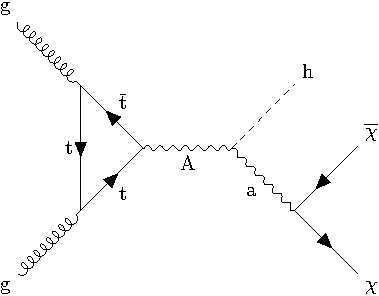
\includegraphics[width=0.525\textwidth]{Chapters/Theory/2HDMa.pdf}
\caption{The pseudoscalar A decaying into a Higgs boson, h, and a pseudoscalar a, which then decays to DM, $\chi$, in the 2HDM+a model.}
\label{fig:2hdma}
\end{figure}

\begin{equation}
    \ptmiss \simeq \frac{\sqrt{(m_\mathrm{A}^2-m_\mathrm{a}^2-m_\mathrm{h}^2)^2-4m_\mathrm{a}^2m_\mathrm{h}^2}}{2m_\mathrm{A}}
    \label{eq:ptmiss}
\end{equation}

Thus, in order to find this peak beyond the typical \ptmiss cut imposed in mono-Higgs searches, it must be that
\begin{equation}
    m_\mathrm{A} \gtrsim m_\mathrm{a} + \sqrt{m_\mathrm{h}^2+({\ptmiss}_{\text{cut}})^2}
\end{equation}

These measurements are expected to be mostly limited by statistical uncertainties through Run 2 of the LHC. As a result, they provide a particularly intriguing avenue to search for DM and are a search that would be interesting to project past the current Phase-1 analyses.

\section{Z\texorpdfstring{$'$}{'} Models}
\label{section:Z'}
Another promising class of simplified dark matter models are ones that propose an additional neutral vector mediator, typically referred to as \Zp. One particular \Zp model that has been investigated recently is the "baryonic Z" model~\cite{barZ2014}. In this model, the baryon number $B$ is gauged and \Zp is a gauge boson of a $U(1)_B$ symmetry. Adding this symmetry would predict additional stable baryons that would make ideal DM candidates. This theory would add interactions between fermionic DM and the SM by adding the following terms to the SM Lagrangian density
\begin{equation}
    g_q\bar{q}\gamma^\mu q\Zp_\mu + g_\chi\bar{\chi}\gamma^\mu\chi\Zp_\mu
\end{equation}

where $g_q = g_B/3$ and $g_\chi = B_\chi g_B$ with $g_B$ as the $U(1)_B$ gauge coupling and $B_\chi$ as the baryon number of the DM candidate. Notably, \Zp does not couple with leptons.

Similar to the Standard Model, the $U(1)_B$ symmetry is broken by a Higgs mechanism, which gives mass to the \Zp boson and leaves a physical particle, the baryonic Higgs h$_B$. There is an interaction between the baryonic Higgs and the baryonic Z, which adds the following term to the SM Lagrangian density
\begin{equation}
    \frac{1}{2}m_\Zp^2(1+\frac{h_B}{v_B})^2\Zp_\mu\Zp^\mu
\end{equation}
where $v_B$ is the VEV of the baryonic Higgs field and $m_\Zp$ is the \Zp mass. h$_B$ also mixes with the SM Higgs, given by the following Lagrangian density term
\begin{equation}
    \frac{m_\Zp^2\sin\zeta}{v_B}
\end{equation}
where $\zeta$ is the h-h$_B$ mixing angle. 

In total, this model has six parameters: $g_q$, $g_\chi$, $m_\Zp$, $m_\chi$, $v_B$, and $\zeta$. Similar to the 2HDM+a model, a variety of searches can provide constraints on the parameter space. In particular, searches that probe a variety of mono-Higgs and \ptmiss final states can provide constraints on the model parameters.

There are also \Zp models that incorporate elements of 2HDMs. One proposal suggests an extension of the SM by a $U(1)_\Zp$ symmetry with a \Zp gauge boson~\cite{Z2hdm2014}. Additionally, there are two Higgs doublets in this model, which behave in an analogous manner to the doublets in the 2HDM+a model, leading to the rise of five bosons: H, h, A$^0$, and H$^\pm$. The A$^0$ boson couples with fermionic DM, while the Higgs mechanism leads to mixing between the Z and \Zp mass states. 

The parameters of this model are the mixing angles $\beta$ and $\alpha$; the masses of the introduced particles $m_\Zp$, $m_\mathrm{h}$, $m_\mathrm{H}$, $m_{\mathrm{A}^0}$, $m_{\mathrm{H}^\pm}$, and $m_\chi$; and the couplings $g_\Zp$ and $g_\chi$. However, in the alignment limit, described previously, $m_\mathrm{h}$ is taken to be that of the SM Higgs and $\alpha = \beta-\frac{\pi}{2}$. Once again, mono-Higgs final states can lead to constraints on these parameters, although this model also has additional constraints from electroweak precision measurements and di-jet final states.